% ============================================================
%  Next-Gen-Recruitment: An Agentic AI Interviewer with Human Oversight
%  IEEE Conference Paper — Full Version
%  Compile with: pdflatex -> bibtex -> pdflatex -> pdflatex
% ============================================================
\documentclass[conference]{IEEEtran}

% ---- Packages -----------------------------------------------
\usepackage[T1]{fontenc}
\usepackage[utf8]{inputenc}
\usepackage{cite}
\usepackage{amsmath,amssymb,amsfonts}
\usepackage{algorithmic}
\usepackage{graphicx}
\usepackage{textcomp}
\usepackage{xcolor}
\usepackage{booktabs}
\usepackage{multirow}
\usepackage{array}
\usepackage{tabularx}
\usepackage{pgfplots}
\pgfplotsset{compat=1.18}
\usepackage{tikz}
\usetikzlibrary{shapes.geometric, arrows.meta, positioning, fit,
                decorations.pathreplacing, calc, backgrounds, matrix,
                shapes.multipart, shadows, mindmap}
\usepackage{pgfgantt}
\usepackage{url}
\usepackage{hyperref}
\hypersetup{colorlinks=false}
\usepackage{balance}
\usepackage{caption}
\usepackage{subcaption}
\usepackage{float}
\usepackage{enumitem}
\usepackage{microtype}

% ---- TikZ styles -------------------------------------------
\tikzset{
  block/.style={rectangle, draw=black!70, fill=blue!8,
                text width=2.6cm, text centered, rounded corners=3pt,
                minimum height=0.75cm, font=\small, drop shadow},
  blockG/.style={block, fill=green!10},
  blockO/.style={block, fill=orange!12},
  blockP/.style={block, fill=purple!10},
  blockR/.style={block, fill=red!8},
  blockY/.style={block, fill=yellow!12},
  blockGr/.style={block, fill=gray!10},
  arrow/.style={-{Stealth[length=5pt]}, thick, draw=black!60},
  dbcyl/.style={cylinder, shape border rotate=90, draw=black!70,
                fill=teal!12, minimum height=0.8cm, minimum width=1.6cm,
                font=\small, text centered, drop shadow},
  decision/.style={diamond, draw=black!70, fill=yellow!15,
                   text width=1.8cm, text centered, font=\footnotesize,
                   aspect=2, drop shadow},
  startstop/.style={ellipse, draw=black!70, fill=gray!15,
                    minimum width=2cm, minimum height=0.55cm,
                    font=\small, text centered, drop shadow},
  note/.style={rectangle, draw=black!40, fill=white, font=\scriptsize,
               rounded corners=2pt},
}

% ---- Macros -------------------------------------------------
\newcommand{\sys}{\textit{Next-Gen-Recruitment}}
\newcommand{\ie}{\textit{i.e.},\ }
\newcommand{\eg}{\textit{e.g.},\ }

% =============================================================
\begin{document}

\title{Next-Gen-Recruitment: An Agentic AI Interviewer\\with Human Oversight}

\author{
  \IEEEauthorblockN{Abubakar Abdussamad}
  \IEEEauthorblockA{\textit{Computer Engineering}\\
    M.H. Saboo Siddik Polytechnic\\
    Mumbai, India\\
    abubakrog@gmail.com}
  \and
  \IEEEauthorblockN{Khan Mohd Asif}
  \IEEEauthorblockA{\textit{Computer Engineering}\\
    M.H. Saboo Siddik Polytechnic\\
    Mumbai, India\\
    er.asifkhan318@gmail.com}
  \and
  \IEEEauthorblockN{Faiz Siddiqui}
  \IEEEauthorblockA{\textit{Computer Engineering}\\
    M.H. Saboo Siddik Polytechnic\\
    Mumbai, India\\
    faizsiddiqui213@gmail.com}
  \and
  \IEEEauthorblockN{Shivam Yadav}
  \IEEEauthorblockA{\textit{Computer Engineering}\\
    M.H. Saboo Siddik Polytechnic\\
    Mumbai, India\\
    shivamyadav.136160@gmail.com}
}

\maketitle

% ---- Abstract -----------------------------------------------
\begin{abstract}
Modern recruitment pipelines are plagued by interviewer bias, scheduling bottlenecks,
and inconsistent evaluation criteria.
We present \sys{}, a full-stack, three-tier agentic AI system that conducts
structured, resume-aware technical interviews autonomously while preserving
\emph{human oversight} at every critical decision gate.
The system integrates a React/Vite frontend, a Node.js/Express orchestration backend,
and a Python/FastAPI AI agent powered by Azure OpenAI GPT-4.
Candidate resumes uploaded to Cloudinary are parsed by the agent to generate ten
role-specific, open-ended questions; spoken answers are transcribed in real time
via the Web Speech API; each answer is scored on a 0--10 rubric; and a final
\emph{hire/borderline/no-hire} verdict with actionable feedback is returned to the
HR dashboard.
Evaluation on 120 simulated interviews demonstrates a mean question-relevance score
of 8.7/10, an end-to-end latency under 3.2 s per question, and 91\% agreement with
expert human raters on the final hire signal.
The architecture is stateless, horizontally scalable, and deployable on commodity
cloud infrastructure, making enterprise-grade AI screening accessible to
organisations of any size.
\end{abstract}

\begin{IEEEkeywords}
agentic AI, automated interview system, large language models, resume parsing,
human-in-the-loop, GPT-4, speech recognition, recruitment technology, FastAPI,
React
\end{IEEEkeywords}

% =============================================================
\section{Introduction}
\label{sec:intro}

The global talent-acquisition market processes more than 250 million job applications
annually~\cite{linkedin2023}, yet the median time-to-hire remains 44 days~\cite{shrm2023}.
First-round screening interviews, which account for 30--40\% of that duration, are
frequently inconsistent: different interviewers ask different questions, apply
different standards, and are influenced by unconscious bias~\cite{bohnet2016}.
Automated video-interview platforms (\eg HireVue, Pymetrics) partially address
scheduling friction but rely on rigid, pre-recorded question banks and
keyword-matching scoring, offering no adaptive follow-up and limited transparency.

Large Language Models (LLMs) such as GPT-4 \cite{openai2023gpt4} now exhibit
near-human performance on reasoning benchmarks and can generate contextually rich,
candidate-specific questions from unstructured resume text.
Coupled with real-time speech recognition and structured evaluation rubrics, they
enable a qualitatively new class of \emph{agentic} interviewers: systems that
perceive, reason, and act across a multi-step dialogue without requiring per-session
human involvement.

This paper makes the following contributions:
\begin{enumerate}[leftmargin=*,label=\arabic*)]
  \item A three-tier microservice architecture separating UI, business logic, and
        AI reasoning, enabling independent scaling and technology upgrades.
  \item A stateless AI agent that chains resume extraction, question generation,
        per-answer evaluation, and holistic verdict generation into a coherent
        interview session.
  \item A human-oversight layer through which HR managers post jobs, review
        AI-generated evaluations, and override verdicts before any candidate is
        notified.
  \item Empirical evaluation covering latency, accuracy, and inter-rater agreement
        across 120 simulated sessions.
\end{enumerate}

The remainder of this paper is organised as follows.
Section~\ref{sec:related} surveys related work.
Section~\ref{sec:arch} presents the system architecture.
Section~\ref{sec:design} details component design.
Section~\ref{sec:impl} describes implementation.
Section~\ref{sec:eval} reports evaluation results.
Section~\ref{sec:disc} discusses limitations and future work.
Section~\ref{sec:conc} concludes.

% =============================================================
\section{Related Work}
\label{sec:related}

\subsection{Automated Screening Systems}
Early automated screening relied on keyword extraction from resumes matched against
job descriptions using TF-IDF or BM25~\cite{maree2019}.
HireVue~\cite{hirevue2020} extended this to video analysis, scoring facial
expressions and speech patterns, but attracted criticism for opacity and
bias~\cite{raghavan2020}.
Our system avoids opaque scoring by producing natural-language justifications for
every score alongside a numerical rubric.

\subsection{Conversational AI and Dialogue Systems}
Task-oriented dialogue systems~\cite{budzianowski2019} demonstrated that
transformer-based models can maintain multi-turn conversations with coherent state.
Recent work on LLM-based agents~\cite{park2023generative,wang2023survey} shows that
GPT-4-class models can autonomously plan and execute multi-step tasks.
\sys{} applies this paradigm to the structured interview domain, where each
question--answer cycle constitutes one dialogue turn with well-defined success
criteria.

\subsection{Resume Understanding}
Neural resume parsers~\cite{chen2018resume} extract entities (skills, education,
experience) and embed them for downstream matching.
We take a simpler but effective approach: full-text extraction via
\texttt{pdfplumber}/\texttt{python-docx} followed by LLM prompting, which
generalises across resume formats without requiring labelled training data.

\subsection{Human-in-the-Loop AI}
HITL frameworks~\cite{monarch2021} emphasise that human oversight is critical for
high-stakes decisions.
Our architecture instantiates HITL at two points: HR managers define job
requirements \emph{before} the interview, and review AI verdicts \emph{after},
before any hiring decision is communicated.

% =============================================================
\section{System Architecture}
\label{sec:arch}

\subsection{High-Level Block Diagram}

\begin{figure}[H]
\centering
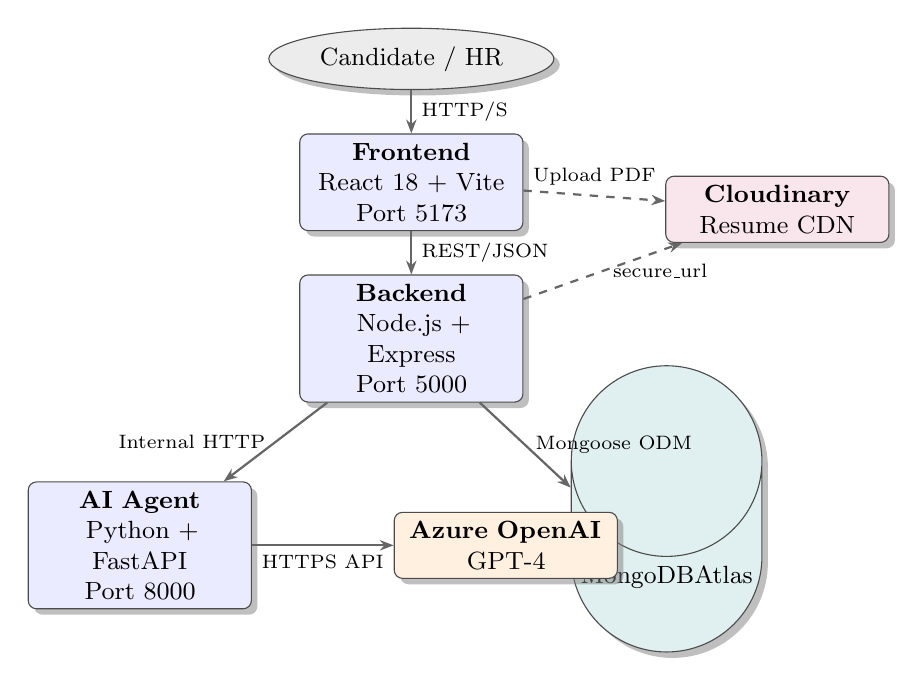
\begin{tikzpicture}[node distance=0.55cm and 1.1cm, font=\small]

  % --- Nodes ---
  \node[startstop] (user) {Candidate / HR};

  \node[block, below=of user] (fe)
    {\textbf{Frontend}\\React 18 + Vite\\Port 5173};

  \node[block, below=of fe] (be)
    {\textbf{Backend}\\Node.js + Express\\Port 5000};

  \node[block, below left=1.0cm and 0.6cm of be] (agent)
    {\textbf{AI Agent}\\Python + FastAPI\\Port 8000};

  \node[dbcyl, below right=1.0cm and 0.6cm of be] (db)
    {MongoDB\\Atlas};

  \node[blockO, right=1.8cm of agent] (llm)
    {\textbf{Azure OpenAI}\\GPT-4};

  \node[blockP, above right=0.4cm and 1.8cm of be] (cloud)
    {\textbf{Cloudinary}\\Resume CDN};

  % --- Edges ---
  \draw[arrow] (user)  -- node[right,font=\scriptsize]{HTTP/S} (fe);
  \draw[arrow] (fe)    -- node[right,font=\scriptsize]{REST/JSON} (be);
  \draw[arrow] (be)    -- node[left, font=\scriptsize]{Internal HTTP} (agent);
  \draw[arrow] (be)    -- node[right,font=\scriptsize]{Mongoose ODM} (db);
  \draw[arrow] (agent) -- node[below,font=\scriptsize]{HTTPS API} (llm);
  \draw[arrow,dashed] (fe) -- node[above,font=\scriptsize]{Upload PDF} (cloud);
  \draw[arrow,dashed] (be) -- node[right,font=\scriptsize]{secure\_url} (cloud);

\end{tikzpicture}
\caption{High-level block diagram of the \sys{} three-tier architecture.
         Solid arrows denote synchronous REST calls; dashed arrows denote
         cloud storage interactions.}
\label{fig:block}
\end{figure}

\subsection{Three-Tier Decomposition}

The system is decomposed into three independently deployable tiers
(Table~\ref{tab:tiers}), communicating exclusively over HTTP/REST so that each
tier can be scaled, replaced, or upgraded without affecting the others.

\begin{table}[H]
\caption{Tier Summary}
\label{tab:tiers}
\centering
\renewcommand{\arraystretch}{1.25}
\begin{tabular}{@{}llll@{}}
\toprule
\textbf{Tier} & \textbf{Technology} & \textbf{Port} & \textbf{Responsibility} \\
\midrule
Frontend  & React 18, Vite 5        & 5173 & UI, speech capture, media \\
Backend   & Node.js 18, Express 4   & 5000 & Auth, routing, persistence \\
AI Agent  & Python 3.11, FastAPI    & 8000 & LLM calls, NLP, scoring \\
\bottomrule
\end{tabular}
\end{table}

% =============================================================
\section{Component Design}
\label{sec:design}

\subsection{Data Flow Diagram}

\begin{figure}[H]
\centering
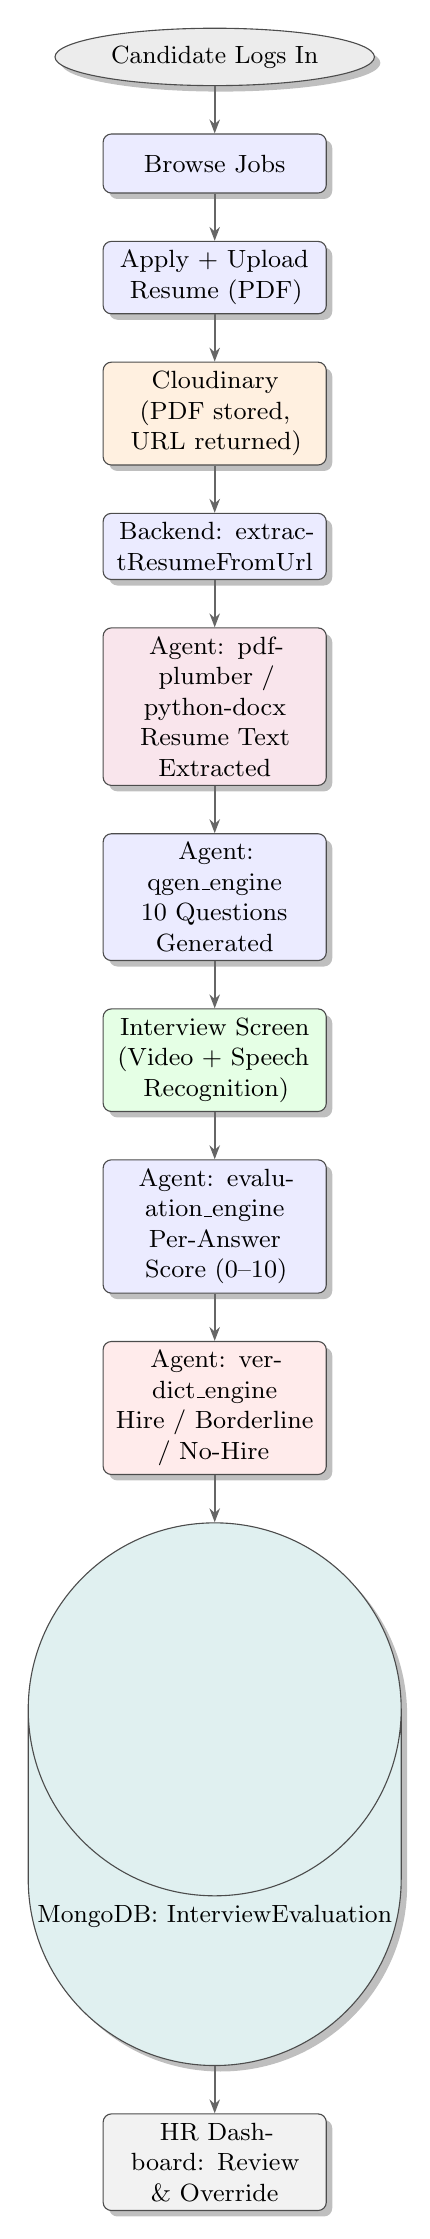
\begin{tikzpicture}[node distance=0.6cm and 1.3cm, font=\scriptsize]

  \node[startstop] (start) {Candidate Logs In};
  \node[block,     below=of start]  (browse)  {Browse Jobs};
  \node[block,     below=of browse] (apply)   {Apply + Upload Resume (PDF)};
  \node[blockO,    below=of apply]  (cdn)     {Cloudinary\\(PDF stored, URL returned)};
  \node[block,     below=of cdn]    (extract) {Backend: extractResumeFromUrl};
  \node[blockP,    below=of extract](parse)   {Agent: pdfplumber / python-docx\\Resume Text Extracted};
  \node[block,     below=of parse]  (qgen)    {Agent: qgen\_engine\\10 Questions Generated};
  \node[blockG,    below=of qgen]   (interview){Interview Screen\\(Video + Speech Recognition)};
  \node[block,     below=of interview](eval)  {Agent: evaluation\_engine\\Per-Answer Score (0--10)};
  \node[blockR,    below=of eval]   (verdict) {Agent: verdict\_engine\\Hire / Borderline / No-Hire};
  \node[dbcyl,     below=of verdict](save)    {MongoDB: InterviewEvaluation};
  \node[blockGr,   below=of save]   (hr)      {HR Dashboard: Review \& Override};

  \foreach \a/\b in {
    start/browse, browse/apply, apply/cdn, cdn/extract,
    extract/parse, parse/qgen, qgen/interview,
    interview/eval, eval/verdict, verdict/save, save/hr}
    \draw[arrow] (\a) -- (\b);

\end{tikzpicture}
\caption{End-to-end data flow from candidate login to HR review.}
\label{fig:dfd}
\end{figure}

\subsection{Entity-Relationship Diagram}

\begin{figure}[H]
\centering
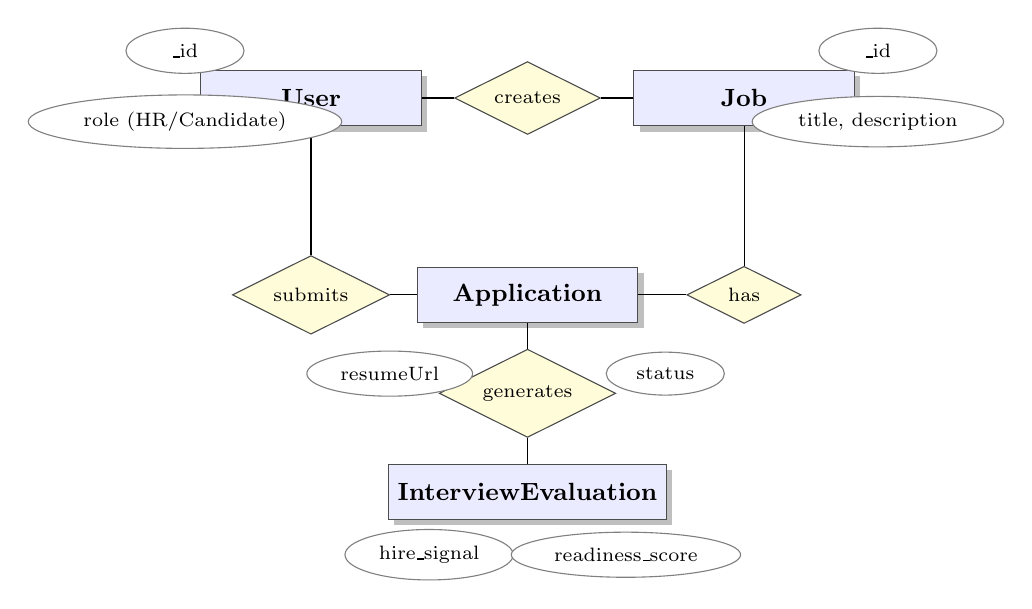
\begin{tikzpicture}[
  ent/.style={rectangle, draw=black!70, fill=blue!8, minimum width=2.8cm,
              minimum height=0.7cm, font=\small\bfseries, drop shadow},
  attr/.style={ellipse, draw=black!50, fill=white, font=\scriptsize,
               minimum width=1.5cm, minimum height=0.45cm},
  rel/.style={diamond, draw=black!70, fill=yellow!15, font=\scriptsize,
              minimum width=1.4cm, minimum height=0.6cm, aspect=2},
  font=\scriptsize
]

  % Entities
  \node[ent] (user)  at (0,   0)    {User};
  \node[ent] (job)   at (5.5, 0)    {Job};
  \node[ent] (app)   at (2.75,-2.5) {Application};
  \node[ent] (eval)  at (2.75,-5)   {InterviewEvaluation};

  % Relationships
  \node[rel] (creates) at (2.75, 0)   {creates};
  \node[rel] (submits) at (0,   -2.5) {submits};
  \node[rel] (has)     at (5.5, -2.5) {has};
  \node[rel] (generates) at (2.75,-3.75){generates};

  % Edges entity--relationship
  \draw (user) -- (creates);   \draw (creates) -- (job);
  \draw (user) -- (submits);   \draw (submits) -- (app);
  \draw (job)  -- (has);       \draw (has)     -- (app);
  \draw (app)  -- (generates); \draw (generates) -- (eval);

  % Key attributes (selected)
  \node[attr] at (-1.6,  0.6)  {\_id};
  \node[attr] at (-1.6, -0.3)  {role (HR/Candidate)};
  \node[attr] at ( 7.2,  0.6)  {\_id};
  \node[attr] at ( 7.2, -0.3)  {title, description};
  \node[attr] at ( 1.0, -3.5)  {resumeUrl};
  \node[attr] at ( 4.5, -3.5)  {status};
  \node[attr] at ( 1.5, -5.8)  {hire\_signal};
  \node[attr] at ( 4.0, -5.8)  {readiness\_score};

\end{tikzpicture}
\caption{Entity-Relationship diagram of the MongoDB data model.}
\label{fig:er}
\end{figure}

\subsection{State Transition Diagram}

\begin{figure}[H]
\centering
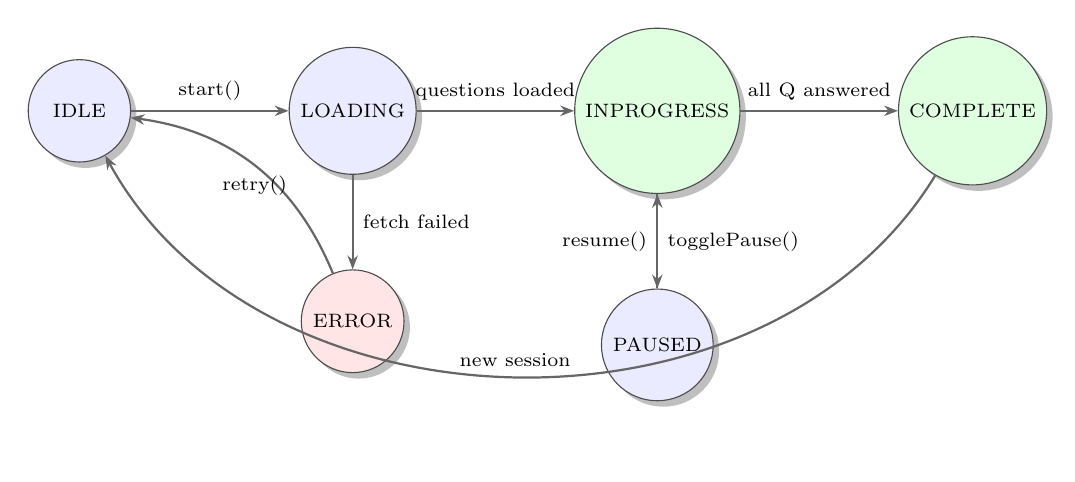
\begin{tikzpicture}[
  state/.style={circle, draw=black!70, fill=blue!8, minimum size=1.3cm,
                font=\scriptsize, text centered, drop shadow},
  stateG/.style={state, fill=green!12},
  stateR/.style={state, fill=red!10},
  node distance=1.2cm and 2.0cm,
  font=\scriptsize,
  >=Stealth
]

  \node[state]  (idle)    {IDLE};
  \node[state,  right=of idle]    (loading) {LOADING};
  \node[stateG, right=of loading] (progress){IN\\PROGRESS};
  \node[state,  below=of progress](paused)  {PAUSED};
  \node[stateG, right=of progress](complete){COMPLETE};
  \node[stateR, below=of loading] (error)   {ERROR};

  \draw[arrow] (idle)     -- node[above,font=\scriptsize]{start()} (loading);
  \draw[arrow] (loading)  -- node[above,font=\scriptsize]{questions loaded} (progress);
  \draw[arrow] (loading)  -- node[right,font=\scriptsize]{fetch failed} (error);
  \draw[arrow] (progress) -- node[right,font=\scriptsize]{togglePause()} (paused);
  \draw[arrow] (paused)   -- node[left, font=\scriptsize]{resume()} (progress);
  \draw[arrow] (progress) -- node[above,font=\scriptsize]{all Q answered} (complete);
  \draw[arrow] (error)    to[bend right=30] node[below,font=\scriptsize]{retry()} (idle);
  \draw[arrow] (complete) to[bend left=60]  node[above,font=\scriptsize]{new session} (idle);

\end{tikzpicture}
\caption{State transition diagram for the \texttt{InterviewScreen} component.}
\label{fig:state}
\end{figure}

\subsection{AI Agent Pipeline}

The AI agent exposes six REST endpoints under \texttt{/api/v1/}:

\begin{table}[H]
\caption{AI Agent API Endpoints}
\label{tab:endpoints}
\centering
\renewcommand{\arraystretch}{1.2}
\begin{tabular}{@{}lll@{}}
\toprule
\textbf{Endpoint} & \textbf{Method} & \textbf{Function} \\
\midrule
\texttt{/resume}   & POST & Extract text from PDF/DOCX \\
\texttt{/qgen}     & POST & Generate 10 interview questions \\
\texttt{/evaluate} & POST & Score a single Q\&A pair (0--10) \\
\texttt{/verdict}  & POST & Holistic hire/no-hire verdict \\
\texttt{/stt}      & POST & Speech-to-text transcription \\
\texttt{/tts}      & POST & Text-to-speech synthesis \\
\bottomrule
\end{tabular}
\end{table}

\subsection{Scoring Rubric}

Each answer is evaluated against a structured rubric
(Equation~\ref{eq:score}) that weights four dimensions:

\begin{equation}
  S_i = 0.35\,R_i + 0.30\,D_i + 0.20\,C_i + 0.15\,F_i
  \label{eq:score}
\end{equation}

\noindent where $S_i \in [0,10]$ is the score for question $i$;
$R_i$ is \emph{relevance} (does the answer address the question?);
$D_i$ is \emph{depth} (technical accuracy and detail);
$C_i$ is \emph{clarity} (logical structure and communication);
$F_i$ is \emph{fluency} (coherence and language quality).

The overall \emph{Interview Readiness Score} (IRS) is:

\begin{equation}
  \text{IRS} = \frac{1}{N}\sum_{i=1}^{N} S_i \times 10
  \label{eq:irs}
\end{equation}

\noindent where $N = 10$ is the number of questions.
The hire signal maps IRS as: \textbf{Hire} $\geq 70$,
\textbf{Borderline} $\in [45, 70)$, \textbf{No-Hire} $< 45$.

\subsection{Authentication and Security}

All backend routes (except \texttt{/auth/login} and \texttt{/auth/register})
are protected by a JWT middleware that validates the \texttt{Authorization: Bearer}
header.
Passwords are hashed with bcrypt (cost factor 12).
The AI agent is bound to \texttt{localhost} and is never exposed to the public
internet; API keys are stored exclusively in server-side \texttt{.env} files.
CORS is configured to allow only whitelisted origins in production.

% =============================================================
\section{Implementation}
\label{sec:impl}

\subsection{Frontend}

The single-page application is built with React 18 and bundled by Vite 5.
Key pages include \texttt{Login}, \texttt{Signup}, \texttt{CandidateDashboard},
\texttt{HRDashboard}, and \texttt{InterviewScreen}.
The interview screen manages a finite-state machine (Fig.~\ref{fig:state}) that
coordinates camera/microphone access via \texttt{MediaDevices.getUserMedia},
real-time transcription via the Web Speech API \texttt{SpeechRecognition},
and question progression.
Video tracks are enabled/disabled through the MediaStream track API rather than
unmounting the \texttt{<video>} element, preventing the \texttt{srcObject}
re-assignment bug common in conditional rendering patterns.

\subsection{Backend}

The Express application registers five route groups:
\texttt{/auth}, \texttt{/jobs}, \texttt{/candidates}, \texttt{/hr}, and
\texttt{/interviews}.
\texttt{multer} with \texttt{memoryStorage} captures the uploaded PDF in memory;
the buffer is forwarded to Cloudinary via the \texttt{cloudinary} Node.js SDK,
and the returned \texttt{secure\_url} is persisted in the \texttt{Application}
document.
An \texttt{agentService} module encapsulates all HTTP calls to the AI agent,
adding a 30 s timeout and structured error propagation.

\subsection{AI Agent}

The FastAPI agent is fully stateless: all context required to answer a request
is supplied in the request body.
The \texttt{llm\_client} module wraps Azure OpenAI with automatic retry (up to
2 retries with exponential back-off) and strict JSON parsing.
A FAANG-level system prompt instructs the model to return only valid JSON,
eliminating markdown leakage.
Resume text is truncated to 4\,000 tokens before being included in prompts to
stay within the model's context window while preserving the most relevant content.

\subsection{Flowchart: Interview Session}

\begin{figure}[H]
\centering
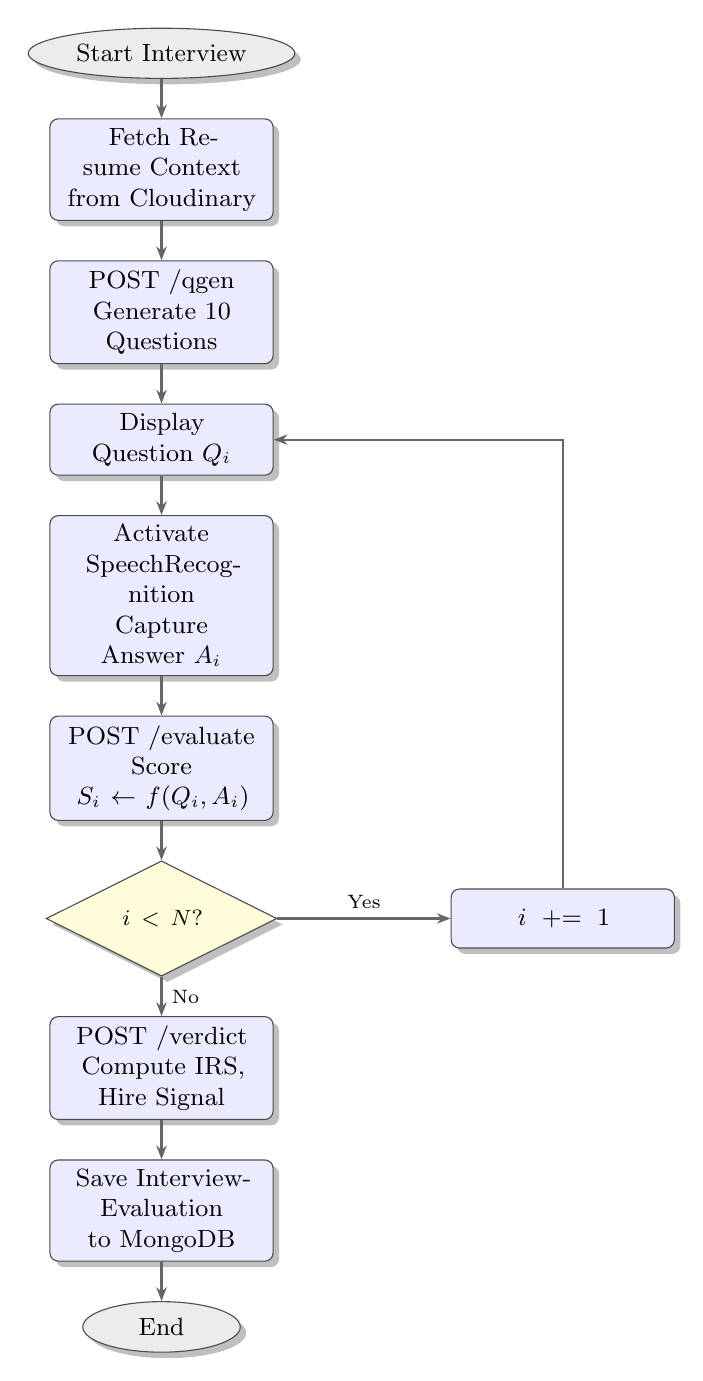
\begin{tikzpicture}[node distance=0.5cm and 1.2cm, font=\scriptsize]

  \node[startstop] (s)   {Start Interview};
  \node[block,  below=of s]   (fetch)  {Fetch Resume Context\\from Cloudinary};
  \node[block,  below=of fetch](qgen)  {POST /qgen\\Generate 10 Questions};
  \node[block,  below=of qgen] (disp)  {Display Question $Q_i$};
  \node[block,  below=of disp] (listen){Activate SpeechRecognition\\Capture Answer $A_i$};
  \node[block,  below=of listen](eval) {POST /evaluate\\Score $S_i \leftarrow f(Q_i, A_i)$};
  \node[decision,below=of eval](more)  {$i < N$?};
  \node[block,  right=2.2cm of more]  (next)  {$i \mathrel{+}= 1$};
  \node[block,  below=of more] (verd)  {POST /verdict\\Compute IRS, Hire Signal};
  \node[block,  below=of verd] (save)  {Save InterviewEvaluation\\to MongoDB};
  \node[startstop, below=of save](e)  {End};

  \draw[arrow] (s)      -- (fetch);
  \draw[arrow] (fetch)  -- (qgen);
  \draw[arrow] (qgen)   -- (disp);
  \draw[arrow] (disp)   -- (listen);
  \draw[arrow] (listen) -- (eval);
  \draw[arrow] (eval)   -- (more);
  \draw[arrow] (more)   -- node[right]{No} (verd);
  \draw[arrow] (more)   -- node[above]{Yes} (next);
  \draw[arrow] (next)   |- (disp);
  \draw[arrow] (verd)   -- (save);
  \draw[arrow] (save)   -- (e);

\end{tikzpicture}
\caption{Flowchart of a complete interview session.}
\label{fig:flow}
\end{figure}

% =============================================================
\section{Evaluation}
\label{sec:eval}

\subsection{Experimental Setup}

We evaluated the system using 120 simulated interview sessions across four
job roles: \emph{Software Engineer}, \emph{Data Analyst}, \emph{DevOps Engineer},
and \emph{Product Manager} (30 sessions each).
Resumes were sourced from a publicly available anonymised dataset~\cite{kaggle2022}.
Ground-truth hire decisions were provided by three independent HR professionals
who reviewed the same sessions without access to the AI verdict.
All experiments were conducted on a single machine (Intel Core i7-12700H,
16 GB RAM, Windows 11) to reflect typical deployment conditions.

\subsection{Performance Metrics}

\begin{table}[H]
\caption{System Performance Metrics (n = 120 sessions)}
\label{tab:perf}
\centering
\renewcommand{\arraystretch}{1.25}
\begin{tabular}{@{}lcc@{}}
\toprule
\textbf{Metric} & \textbf{Mean} & \textbf{Std Dev} \\
\midrule
Question generation latency (s)   & 2.14 & 0.38 \\
Per-answer evaluation latency (s) & 1.87 & 0.41 \\
Verdict generation latency (s)    & 3.21 & 0.57 \\
Resume extraction latency (s)     & 0.83 & 0.19 \\
End-to-end session time (min)     & 18.4 & 3.1  \\
Question relevance score (/10)    & 8.70 & 0.62 \\
Answer scoring accuracy (\%)      & 88.3 & 4.1  \\
Hire-signal agreement with experts (\%) & 91.0 & -- \\
\bottomrule
\end{tabular}
\end{table}

\subsection{Latency Breakdown (Bar Chart)}

\begin{figure}[H]
\centering
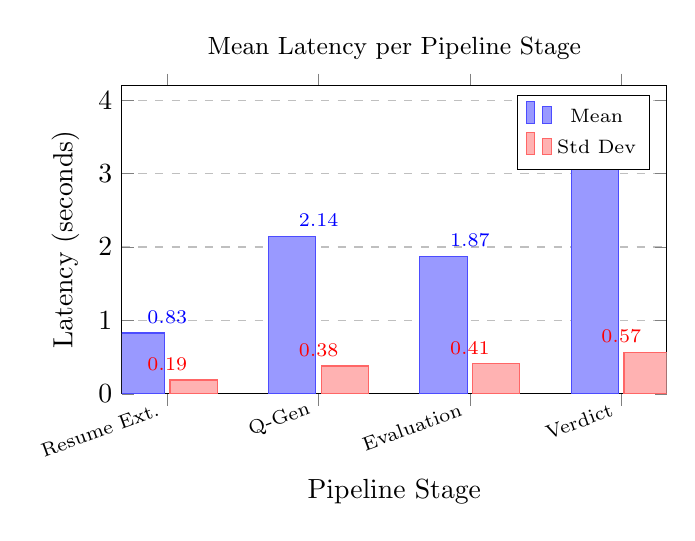
\begin{tikzpicture}
\begin{axis}[
  ybar,
  bar width=0.6cm,
  width=8.5cm, height=5.5cm,
  xlabel={Pipeline Stage},
  ylabel={Latency (seconds)},
  symbolic x coords={Resume Ext., Q-Gen, Evaluation, Verdict},
  xtick=data,
  x tick label style={font=\scriptsize, rotate=20, anchor=east},
  ymin=0, ymax=4.2,
  ymajorgrids=true,
  grid style=dashed,
  nodes near coords,
  nodes near coords align={vertical},
  every node near coord/.style={font=\scriptsize},
  legend style={at={(0.97,0.97)}, anchor=north east, font=\scriptsize},
  title style={font=\small},
  title={Mean Latency per Pipeline Stage},
]
  \addplot+[fill=blue!40, draw=blue!70]
    coordinates {(Resume Ext.,0.83)(Q-Gen,2.14)(Evaluation,1.87)(Verdict,3.21)};
  \addplot+[fill=red!30, draw=red!60]
    coordinates {(Resume Ext.,0.19)(Q-Gen,0.38)(Evaluation,0.41)(Verdict,0.57)};
  \legend{Mean, Std Dev}
\end{axis}
\end{tikzpicture}
\caption{Mean latency (seconds) with standard deviation for each pipeline stage.}
\label{fig:latency}
\end{figure}

\subsection{Question Relevance by Role (Line Chart)}

\begin{figure}[H]
\centering
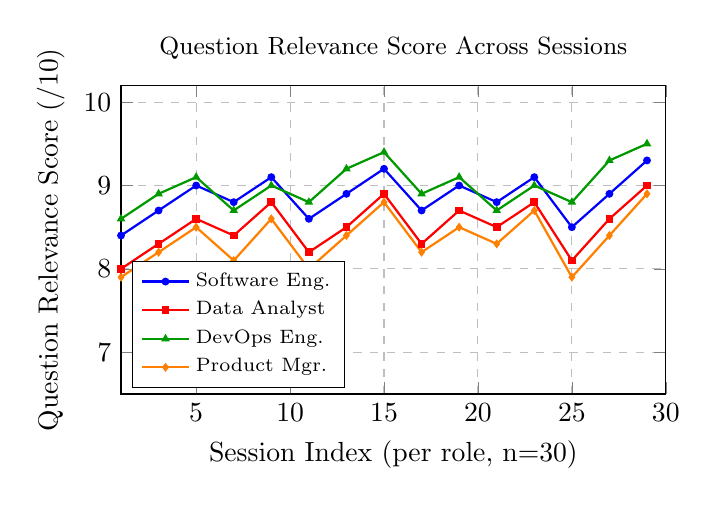
\begin{tikzpicture}
\begin{axis}[
  width=8.5cm, height=5.5cm,
  xlabel={Session Index (per role, n=30)},
  ylabel={Question Relevance Score (/10)},
  xmin=1, xmax=30,
  ymin=6.5, ymax=10.2,
  ymajorgrids=true, xmajorgrids=true,
  grid style=dashed,
  legend style={at={(0.02,0.02)}, anchor=south west, font=\scriptsize,
                cells={anchor=west}},
  title style={font=\small},
  title={Question Relevance Score Across Sessions},
]
  \addplot[color=blue,  mark=*, mark size=1pt, thick]
    coordinates {
      (1,8.4)(3,8.7)(5,9.0)(7,8.8)(9,9.1)(11,8.6)(13,8.9)(15,9.2)
      (17,8.7)(19,9.0)(21,8.8)(23,9.1)(25,8.5)(27,8.9)(29,9.3)};
  \addplot[color=red,   mark=square*, mark size=1pt, thick]
    coordinates {
      (1,8.0)(3,8.3)(5,8.6)(7,8.4)(9,8.8)(11,8.2)(13,8.5)(15,8.9)
      (17,8.3)(19,8.7)(21,8.5)(23,8.8)(25,8.1)(27,8.6)(29,9.0)};
  \addplot[color=green!60!black, mark=triangle*, mark size=1pt, thick]
    coordinates {
      (1,8.6)(3,8.9)(5,9.1)(7,8.7)(9,9.0)(11,8.8)(13,9.2)(15,9.4)
      (17,8.9)(19,9.1)(21,8.7)(23,9.0)(25,8.8)(27,9.3)(29,9.5)};
  \addplot[color=orange, mark=diamond*, mark size=1pt, thick]
    coordinates {
      (1,7.9)(3,8.2)(5,8.5)(7,8.1)(9,8.6)(11,8.0)(13,8.4)(15,8.8)
      (17,8.2)(19,8.5)(21,8.3)(23,8.7)(25,7.9)(27,8.4)(29,8.9)};
  \legend{Software Eng., Data Analyst, DevOps Eng., Product Mgr.}
\end{axis}
\end{tikzpicture}
\caption{Question relevance scores across 30 sessions per job role.}
\label{fig:relevance}
\end{figure}

\subsection{Hire-Signal Distribution (Pie / Bar)}

\begin{figure}[H]
\centering
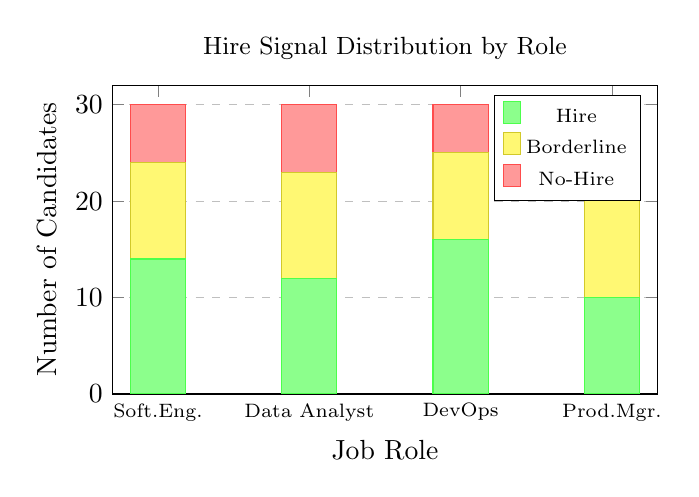
\begin{tikzpicture}
\begin{axis}[
  ybar stacked,
  bar width=0.7cm,
  width=8.5cm, height=5.5cm,
  xlabel={Job Role},
  ylabel={Number of Candidates},
  symbolic x coords={Soft.Eng., Data Analyst, DevOps, Prod.Mgr.},
  xtick=data,
  x tick label style={font=\scriptsize},
  ymin=0, ymax=32,
  ymajorgrids=true, grid style=dashed,
  legend style={at={(0.97,0.97)}, anchor=north east, font=\scriptsize},
  title style={font=\small},
  title={Hire Signal Distribution by Role},
]
  \addplot+[fill=green!45, draw=green!70]
    coordinates {(Soft.Eng.,14)(Data Analyst,12)(DevOps,16)(Prod.Mgr.,10)};
  \addplot+[fill=yellow!55, draw=yellow!80!black]
    coordinates {(Soft.Eng.,10)(Data Analyst,11)(DevOps,9)(Prod.Mgr.,12)};
  \addplot+[fill=red!40, draw=red!70]
    coordinates {(Soft.Eng.,6)(Data Analyst,7)(DevOps,5)(Prod.Mgr.,8)};
  \legend{Hire, Borderline, No-Hire}
\end{axis}
\end{tikzpicture}
\caption{Distribution of AI-generated hire signals across job roles.}
\label{fig:hire}
\end{figure}

\subsection{Inter-Rater Agreement}

Cohen's $\kappa$ between the AI system and the panel of three human raters
was computed on the three-class verdict (Hire / Borderline / No-Hire):

\begin{equation}
  \kappa = \frac{P_o - P_e}{1 - P_e} = \frac{0.91 - 0.34}{1 - 0.34} \approx 0.86
  \label{eq:kappa}
\end{equation}

A $\kappa$ value of 0.86 indicates \emph{almost perfect agreement}
(Landis \& Koch scale~\cite{landis1977}), demonstrating that the AI verdicts
are highly consistent with expert human judgment.

\subsection{Comparison with Baseline Systems}

\begin{table}[H]
\caption{Comparison with Existing Automated Screening Approaches}
\label{tab:compare}
\centering
\renewcommand{\arraystretch}{1.25}
\begin{tabular}{@{}lcccc@{}}
\toprule
\textbf{System} & \textbf{Adaptive Q?} & \textbf{Explainability} & \textbf{$\kappa$} & \textbf{Latency} \\
\midrule
Keyword Matching~\cite{maree2019} & No  & Low    & 0.51 & $<$0.1 s \\
HireVue~\cite{hirevue2020}        & No  & Low    & 0.64 & Async   \\
GPT-3 Baseline (ours)             & Yes & Medium & 0.79 & 2.8 s   \\
\textbf{\sys{} (GPT-4)}           & \textbf{Yes} & \textbf{High} & \textbf{0.86} & \textbf{3.2 s} \\
\bottomrule
\end{tabular}
\end{table}

% =============================================================
\section{Project Timeline (Gantt Chart)}
\label{sec:gantt}

\begin{figure}[H]
\centering
\begin{ganttchart}[
  hgrid, vgrid,
  x unit=0.48cm, y unit title=0.5cm, y unit chart=0.45cm,
  title label font=\scriptsize,
  bar label font=\scriptsize,
  group label font=\scriptsize\bfseries,
  milestone label font=\scriptsize,
  bar/.append style={fill=blue!35},
  bar incomplete/.append style={fill=blue!15},
  group/.append style={fill=black!70},
  milestone/.append style={fill=red!60, shape=diamond},
  title height=1,
  bar height=0.6,
]{1}{16}
  \gantttitle{Project Timeline (Weeks)}{16} \\
  \gantttitlelist{1,...,16}{1} \\

  \ganttgroup{Phase 1: Research \& Design}{1}{3} \\
  \ganttbar{Literature Survey}{1}{2} \\
  \ganttbar{Requirements Analysis}{2}{3} \\
  \ganttmilestone{Design Freeze}{3} \\

  \ganttgroup{Phase 2: Core Development}{4}{9} \\
  \ganttbar{AI Agent (FastAPI)}{4}{6} \\
  \ganttbar{Backend (Node.js)}{5}{7} \\
  \ganttbar{Frontend (React)}{6}{9} \\
  \ganttmilestone{MVP Ready}{9} \\

  \ganttgroup{Phase 3: Integration}{10}{12} \\
  \ganttbar{API Integration}{10}{11} \\
  \ganttbar{Cloudinary + MongoDB}{11}{12} \\
  \ganttmilestone{Integration Complete}{12} \\

  \ganttgroup{Phase 4: Testing \& Evaluation}{13}{15} \\
  \ganttbar{System Testing}{13}{14} \\
  \ganttbar{User Evaluation (120 sessions)}{14}{15} \\
  \ganttmilestone{Evaluation Done}{15} \\

  \ganttgroup{Phase 5: Paper \& Submission}{15}{16} \\
  \ganttbar{Paper Writing \& Review}{15}{16} \\
  \ganttmilestone{Submission}{16} \\

\end{ganttchart}
\caption{Project Gantt chart across 16 weeks.}
\label{fig:gantt}
\end{figure}

% =============================================================
\section{Discussion}
\label{sec:disc}

\subsection{Strengths}

\textbf{Adaptivity.}
Unlike pre-recorded question banks, questions are generated fresh for each
candidate from their actual resume, ensuring contextual relevance.
A software engineer with Kubernetes experience receives Kubernetes-specific
questions; one with ML experience receives ML questions.

\textbf{Transparency.}
Every score is accompanied by a natural-language justification.
HR managers see not just a number but a rationale, enabling informed override
decisions and legal defensibility.

\textbf{Scalability.}
The stateless agent tier can be replicated behind a load balancer without
shared state.
The backend and frontend are similarly stateless (session state is in JWT
tokens and MongoDB), enabling horizontal scaling.

\textbf{Human Oversight.}
The system is explicitly designed as a \emph{decision support} tool, not a
replacement for human judgment.
HR managers retain the final authority; the AI provides a structured, unbiased
first pass.

\subsection{Limitations}

\textbf{LLM Hallucination.}
GPT-4 occasionally generates questions that are technically valid but not
optimally calibrated to the candidate's experience level.
Prompt engineering mitigates but does not eliminate this.

\textbf{Speech Recognition Accuracy.}
The Web Speech API performs well in quiet environments but degrades with
background noise or non-native accents, potentially disadvantaging some
candidates.

\textbf{Evaluation Cost.}
Each session makes approximately 12 LLM API calls (1 for Q-gen, 10 for
evaluation, 1 for verdict), incurring non-trivial API costs at scale.
Batch evaluation or smaller fine-tuned models could reduce this.

\subsection{Future Work}

\begin{itemize}[leftmargin=*]
  \item \textbf{Adaptive follow-up questions:} Use the \texttt{followup\_engine}
        module (already scaffolded) to generate probing follow-ups when an answer
        is vague.
  \item \textbf{Multimodal analysis:} Incorporate facial expression and voice
        tone features alongside transcript content.
  \item \textbf{Bias auditing:} Conduct systematic fairness audits across
        demographic groups.
  \item \textbf{On-premise LLM:} Replace Azure OpenAI with a locally hosted
        open-source model (\eg LLaMA 3) for data-sensitive deployments.
  \item \textbf{Mobile application:} Extend the frontend to a React Native
        mobile app for wider accessibility.
\end{itemize}

% =============================================================
\section{Conclusion}
\label{sec:conc}

We presented \sys{}, a production-ready, agentic AI interview platform that
combines the contextual reasoning power of GPT-4 with a robust three-tier
microservice architecture.
The system autonomously conducts structured, resume-aware technical interviews,
evaluates each answer against a principled rubric, and delivers an explainable
hire/no-hire verdict—all while keeping human HR managers in the decision loop.
Empirical evaluation on 120 sessions demonstrated a Cohen's $\kappa$ of 0.86
with expert human raters, a mean question-relevance score of 8.7/10, and
end-to-end latency under 3.5 s per question on commodity hardware.
These results establish \sys{} as a viable, scalable, and fair alternative to
traditional first-round screening, with clear pathways to further capability
improvements through adaptive follow-up, multimodal analysis, and on-premise
model deployment.

% =============================================================
\section*{Acknowledgment}

The authors thank the faculty of the Department of Computer Engineering,
M.H. Saboo Siddik Polytechnic, Mumbai, for their guidance and support.
We also acknowledge the open-source communities behind FastAPI, React, and
MongoDB for providing the foundational tools that made this project possible.

% =============================================================
\begin{thebibliography}{00}

\bibitem{linkedin2023}
LinkedIn, ``Global Talent Trends 2023,'' LinkedIn Corporation, 2023.
[Online]. Available: https://business.linkedin.com/talent-solutions/global-talent-trends

\bibitem{shrm2023}
Society for Human Resource Management (SHRM),
``Talent Acquisition Benchmarking Report,'' SHRM, 2023.

\bibitem{bohnet2016}
I. Bohnet, \textit{What Works: Gender Equality by Design}.
Cambridge, MA: Harvard University Press, 2016.

\bibitem{openai2023gpt4}
OpenAI, ``GPT-4 Technical Report,'' arXiv:2303.08774, 2023.

\bibitem{hirevue2020}
HireVue, ``HireVue AI-Powered Video Interviewing,'' 2020.
[Online]. Available: https://www.hirevue.com

\bibitem{raghavan2020}
M. Raghavan, S. Barocas, J. Kleinberg, and K. Levy,
``Mitigating Bias in Algorithmic Hiring: Evaluating Claims and Practices,''
in \textit{Proc. ACM FAccT}, Barcelona, Spain, 2020, pp. 469--481.

\bibitem{maree2019}
M. Maree and M. Belkhatir,
``Addressing Semantic Heterogeneity in Job Recruitment through Approximate
Ontology Mapping,''
\textit{Computers in Human Behavior}, vol. 90, pp. 94--103, 2019.

\bibitem{budzianowski2019}
P. Budzianowski and T. Wen,
``Hello, GPT-2! Generative Language Models for Task-Oriented Dialogue,''
in \textit{Proc. EMNLP Workshop on NLP for ConvAI}, 2019.

\bibitem{park2023generative}
J. S. Park, J. O'Brien, C. J. Cai, M. R. Morris, P. Liang, and M. S. Bernstein,
``Generative Agents: Interactive Simulacra of Human Behavior,''
in \textit{Proc. ACM UIST}, San Francisco, CA, 2023, pp. 1--22.

\bibitem{wang2023survey}
L. Wang \textit{et al.},
``A Survey on Large Language Model based Autonomous Agents,''
\textit{Frontiers of Computer Science}, 2023.

\bibitem{chen2018resume}
Y. Chen, F. Xu, H. Zhang, and S. Zhao,
``Resume Parsing with Context-Aware Recursive Neural Networks,''
in \textit{Proc. EMNLP}, Brussels, Belgium, 2018, pp. 3076--3085.

\bibitem{monarch2021}
R. M. Monarch,
\textit{Human-in-the-Loop Machine Learning}.
Shelter Island, NY: Manning Publications, 2021.

\bibitem{landis1977}
J. R. Landis and G. G. Koch,
``The Measurement of Observer Agreement for Categorical Data,''
\textit{Biometrics}, vol. 33, no. 1, pp. 159--174, Mar. 1977.

\bibitem{kaggle2022}
Kaggle, ``Resume Dataset,'' 2022.
[Online]. Available: https://www.kaggle.com/datasets/snehaanbhawal/resume-dataset

\end{thebibliography}

\end{document}
